\hspace{4mm}Afin de finaliser notre projet la partie réalisation est d'autant plus importante que la phase de conception. Dans ce chapitre nous allons tout d'abord décrire les outils de développement adoptés pour la réalisation de notre application. Ensuite nous présenterons quelques interfaces de l'application.
\section{	Environnement de travail}
\subsection{	Environnement logiciel }
\subsubsection{	Outils logiciels}
\begin{itemize}
    \item 	Spring Tool Suite 
\end{itemize}
\par Spring Tool Suite est un IDE pour développer des applications Spring. Il s'agit d'un environnement de développement basé sur Eclipse. Il fournit un environnement prêt à l'emploi pour implémenter, exécuter, déployer et déboguer l'application. Il valide notre application et fournit des correctifs rapides pour les applications. \cite{5}
\newline
\begin{figure}[h]
    \centering
    
\includegraphics[scale=0.5]{figures/3333anis5.png}
    \caption*{}
    \label{fig:logo_STS}
\end{figure}\newpage
\begin{itemize}
    \item 	Visual Studio
\end{itemize}
\par Visual Studio Code est un éditeur du code léger et puissant supportant le travail avec TypeScript et Angular. Il dispose d’un éco système riche d’extensions qui nous a énormément aidés au cours du développement de notre application Web \cite{6}.
\begin{figure}[h]
    \centering
    
\includegraphics{figures/33anis6.png}
    \caption*{}
    \label{fig:logo_VS}
\end{figure}
\begin{itemize}
    \item 	Postman 
\end{itemize}
\par C’est une plateforme de collaboration qui se focalise sur les tests des APIs. Nous l’avons utilisé pour tester nos propres APIs \cite{7}.
\begin{figure}[h]
    \centering
    
\includegraphics{figures/33anis7.png}
    \caption*{}
    \label{fig:logo_POSTMAN}
\end{figure}
\begin{itemize}
    \item 	Gitlab 
\end{itemize}
\par GitLab est la première et unique application pour le développement, la sécurité et l’exploitation de logiciels, prenant en charge les DevOps simultanés. Elle permet d’accélérer ainsi le cycle de vie du logiciel et augmenter la vitesse de l’entreprise \cite{8}.
\begin{figure}[h]
    \centering
    
\includegraphics[scale=0.08]{figures/3333anis6.png}
    \caption*{}
    \label{fig:logo_GITLAB}
\end{figure}\newpage
\subsubsection{	Technologies}
\begin{itemize}
    \item 	Angular 
\end{itemize}
\par Il s’agit d’un framework développé et maintenu par Google. Il est basé sur le langage TypeScript et optimisé pour les applications Web composées d’une seule page côté client. Il est utilisé pour développer une interface client mono-page extrêmement robuste et adaptable \cite{9}.
\begin{figure}[h]
    \centering
    
\includegraphics{figures/33anis9.png}
    \caption*{}
    \label{fig:logo_ANGULAR}
\end{figure}
\begin{itemize}
    \item	Spring Boot 
\end{itemize}
\par Spring Boot est un framework open source, basé sur Java et utilisé dans la création de microservices. Il a été développé par Pivotal Team pour créer des applications Spring indépendantes et prêtes pour la production \cite{5}. 
\begin{figure}[h]
    \centering
    
\includegraphics{figures/33anis10.png}
    \caption*{}
    \label{fig:logo_SPRINGB}
\end{figure}
\begin{itemize}
    \item	Spring Security
\end{itemize}
\par Spring Security est un framework qui fournit l’authentification et d’autres fonctionnalités de sécurité pour les applications Java \cite{5}.
\begin{figure}[h]
    \centering
    
\includegraphics{figures/33anis11.png}
    \caption*{}
    \label{fig:logo_SPRINGS}
\end{figure}
\begin{itemize}
    \item	TypeScript
\end{itemize}
\par TypeScript est un langage de programmation libre et open source développé par Microsoft qui a pour but d'améliorer et de sécuriser la production de code JavaScript. \cite{10}
\begin{figure}[h]
    \centering
    
\includegraphics{figures/33anis13.png}
    \caption*{}
    \label{fig:logo_TYPES}
\end{figure}
\begin{itemize}
    \item	PostgreSQL
\end{itemize}
\par Est un puissant système de base de données relationnelle objet open source avec plus de 30 ans de développement actif qui lui a valu une solide réputation de fiabilité, de robustesse des fonctionnalités et de performances. \cite{11}
\begin{figure}[h]
    \centering
    
\includegraphics{figures/33anis14.png}
    \caption*{}
    \label{fig:logo_POSTGRE}
\end{figure}
\subsection{	Environnement matériel}
\begin{itemize}
    \item 	Ordinateurs portables
    \begin{itemize}
        \item DELL LATITUDE | E5510 ayant les caractéristiques suivantes :
        \begin{itemize}
            \item	Processeur Intel® Core™ i5 CPU M560 @ 2.67GHz, 2.67 GHz.
            \item 	Mémoire installée : 8Go, Disque dur SSD: 300 Go.
            \item	Système d’exploitation : Windows 10, 64 bits.
        \end{itemize}
    \end{itemize}
\end{itemize}\newpage
\section{	Interface de l'application}
\hspace{4mm}Cette partie détaillera la solution finale obtenue. Ainsi, nous présentons notre application à travers des imprimés écrans correspondants au travail réalisé.
\subsection{	Interfaces de souscription}
\hspace{4mm}Cette interface permet à l’utilisateur de choisir l’offre d’inscription.
\begin{figure}[h]
    \centering
    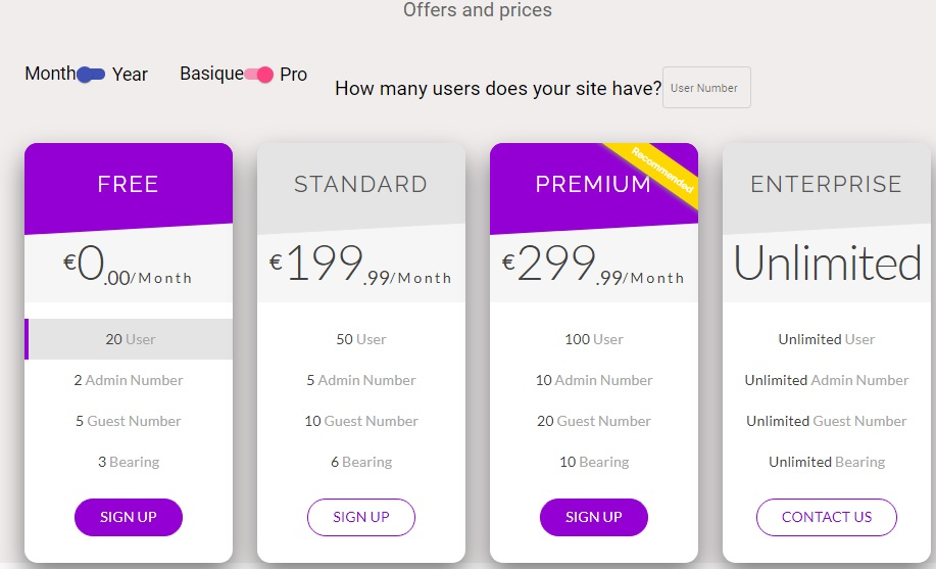
\includegraphics{figures/33anis15.png}
    \caption{Interface de sélection de l’offre d’inscription}
    \label{fig:interface_offre}
\end{figure}
\par La figure suivante présente l’interface d’inscription. L’utilisateur doit saisir son e-mail pour recevoir un mail d’activation. Une fois qu’on clique sur le lien reçu sur l’e-mail, le compte va être activé.\newpage
\begin{figure}[h]
    \centering
    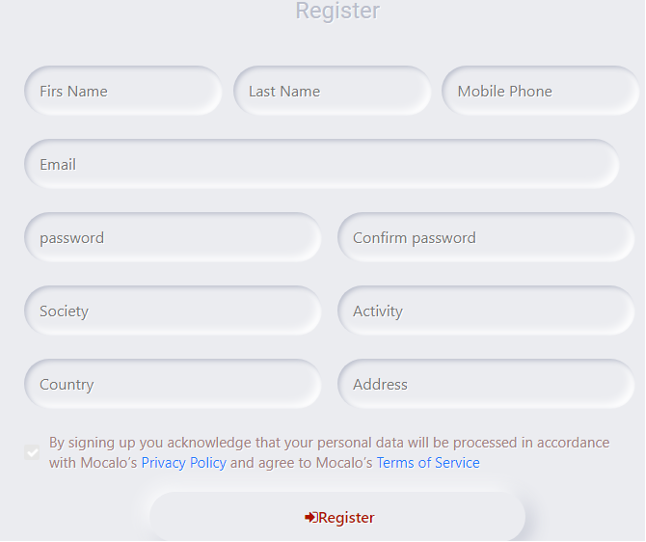
\includegraphics{figures/33anis16.png}
    \caption{Interface d’inscription}
    \label{fig:interface_inscri}
\end{figure}
\subsection{	Interface d’authentification}
\hspace{4mm}La figure \ref{fig:interface_auth} ci-dessous illustre l’interface d’accès à l’application. Elle implémente la fonction qui consiste à vérifier l’identité de l’utilisateur par un login et un mot de passe, afin de lui autoriser l’accès à cette application et lui offrir les services dédiés à son profil.
\begin{figure}[h]
    \centering
    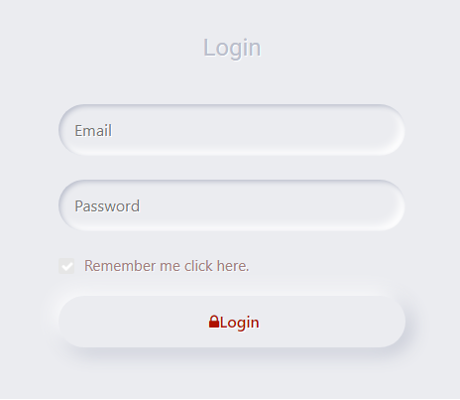
\includegraphics{figures/33anis17.png}
    \caption{Interface d’authentification}
    \label{fig:interface_auth}
\end{figure}
\subsection{	Interface de Dashboard}
\hspace{4mm}La figure ci-dessous \ref{fig:interface_dashb} présente l’interface de Dashboard, où l’utilisateur est en mesure de consulter les détails de tous les projets, les tâches et les anomalies. Il a  aussi la main pour gérer soit par ajout ou par modification  s’il a le droit. 
\newline
\begin{figure}[h]
    \centering
    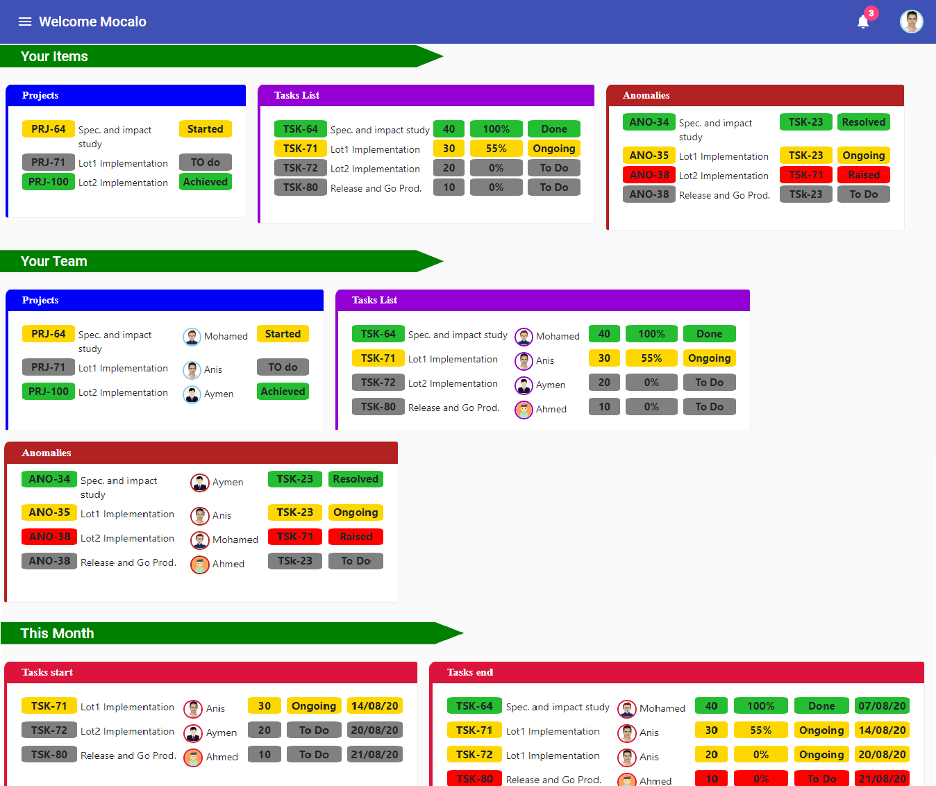
\includegraphics{figures/33anis18.png}
    \caption{Interface de Dashboard}
    \label{fig:interface_dashb}
\end{figure}\newpage
\subsection{	Interface d’une équipe}
\hspace{4mm}La figure ci-dessous \ref{fig:interface_équipe} présente l’interface d’une équipe sélectionnée, où l’utilisateur est en mesure de consulter les détails de tous les projets, les tâches et les anomalies pour une équipe sélectionnée. Cette interface offre aussi la possibilité de consulter la liste de ses membres.\newline
\begin{figure}[h]
    \centering
    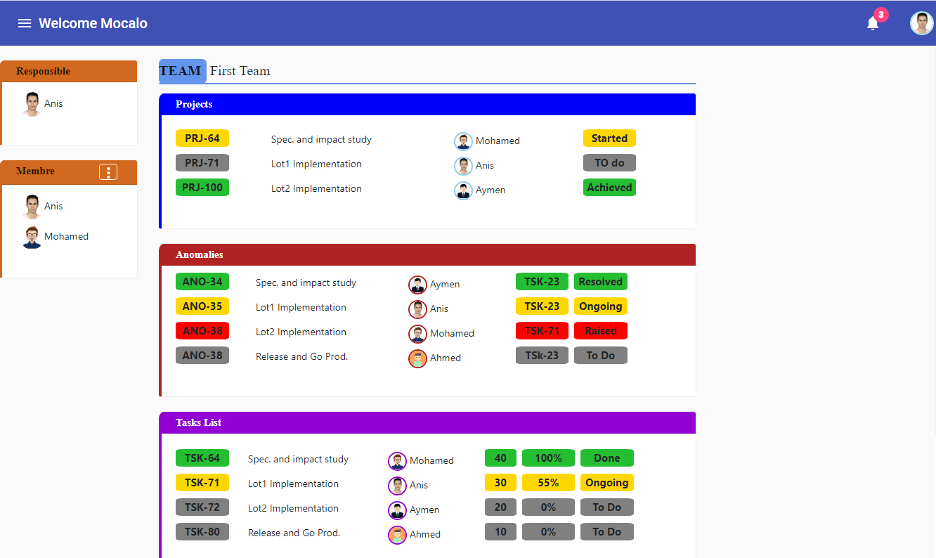
\includegraphics{figures/33anis19.png}
    \caption{Interface d’une équipe}
    \label{fig:interface_équipe}
\end{figure}\newpage
\subsection{	Interface d’un projet}
\hspace{4mm}La figure suivante présente les détails d’un projet. Cette interface offre aussi la possibilité de consulter la liste de ses titulaires de droits, la liste de ses observateurs, la liste de ses donneurs de go, la liste de ses tâches, les détails de ses planifications et les détails de ses risques.
\begin{figure}[h]
    \centering
    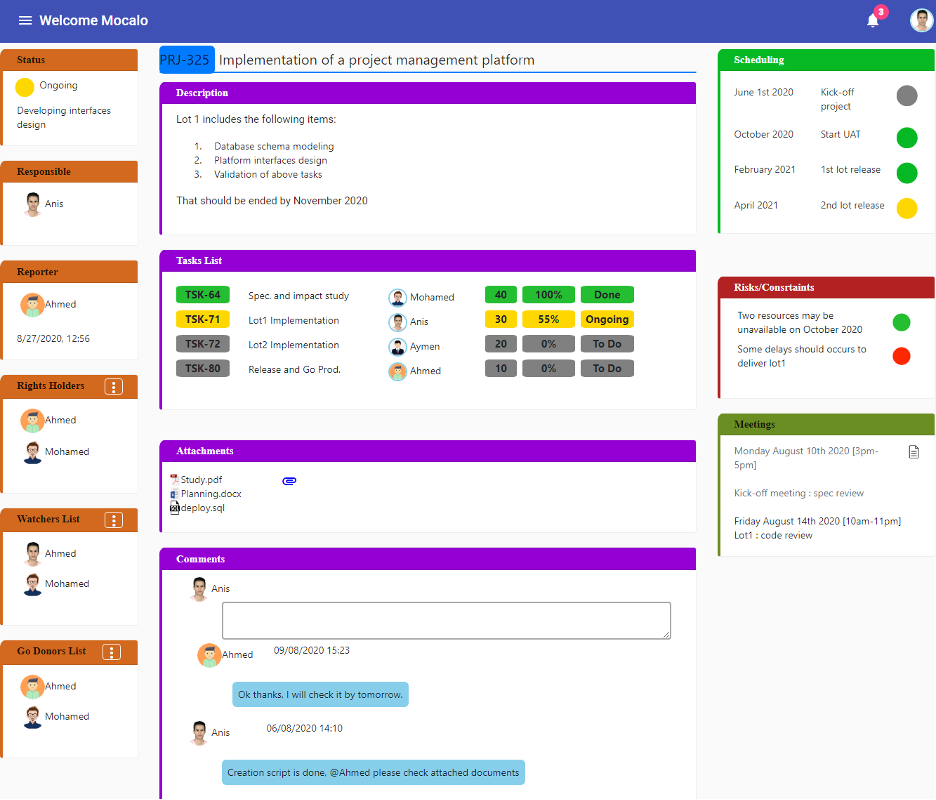
\includegraphics{figures/33anis20.png}
    \caption{Interface d’un projet}
    \label{fig:interface_projet}
\end{figure}\newpage
\subsubsection{	Interface de la liste des titulaires de droits }
\hspace{4mm}La figure suivante présente l’interface de la liste des titulaires de droits sur le projet.
\begin{figure}[h]
    \centering
    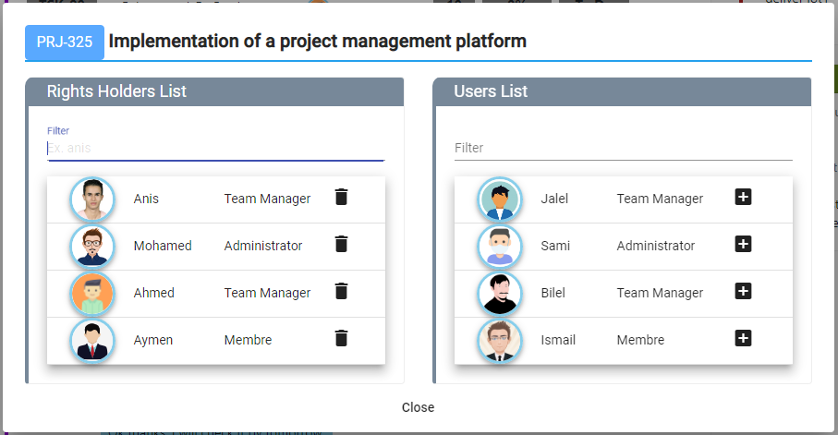
\includegraphics{figures/33anis21.png}
    \caption{Interface de la liste des titulaires de droits}
    \label{fig:interface_titulaires}
\end{figure}
\subsubsection{Interface de la liste des observateurs }
\hspace{4mm}La figure suivante présente l’interface de la liste des observateurs sur le projet.
\begin{figure}[h]
    \centering
    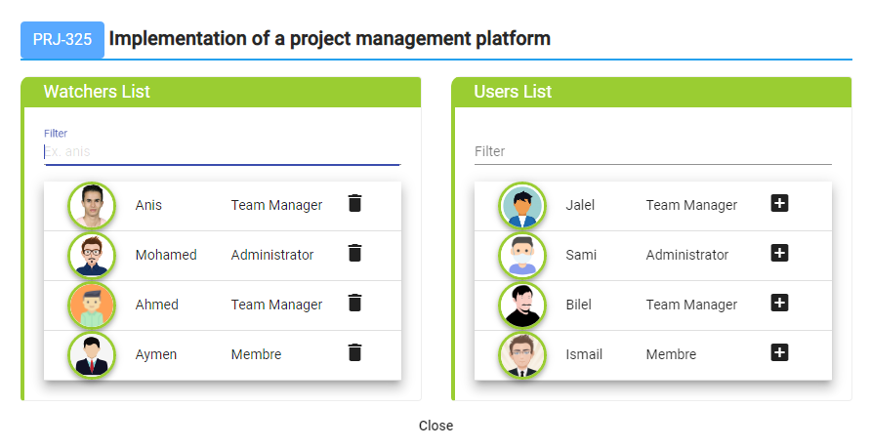
\includegraphics{figures/33anis22.png}
    \caption{Interface de la liste des observateurs}
    \label{fig:interface_observateur}
\end{figure}\newpage
\subsubsection{Interface de la liste des donneurs de go }
\hspace{4mm}La figure suivante présente l’interface de la liste des donneurs de go sur le projet.
\begin{figure}[h]
    \centering
    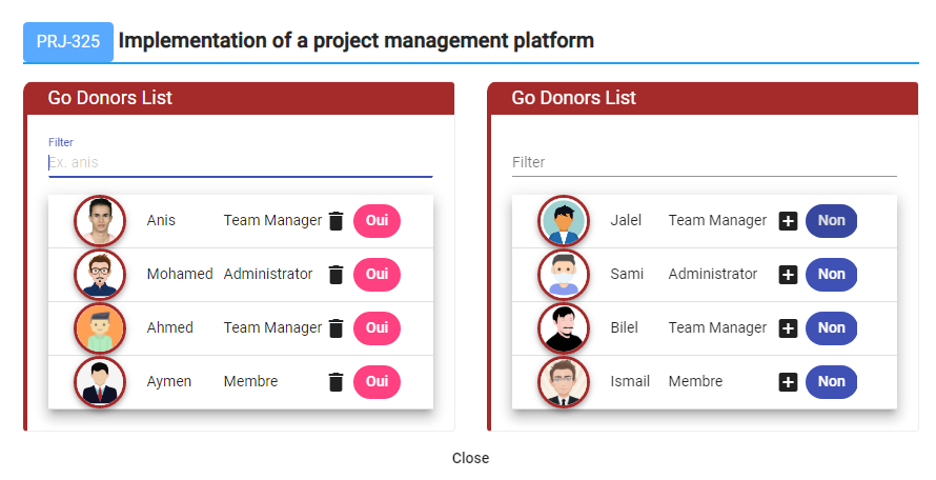
\includegraphics{figures/33anis23.png}
    \caption{Interface de la liste des donneurs de go}
    \label{fig:interface_donneur}
\end{figure}
\subsubsection{Interface de planification}
\hspace{4mm}La figure suivante présente les détails d’une planification.
\begin{figure}[h]
    \centering
    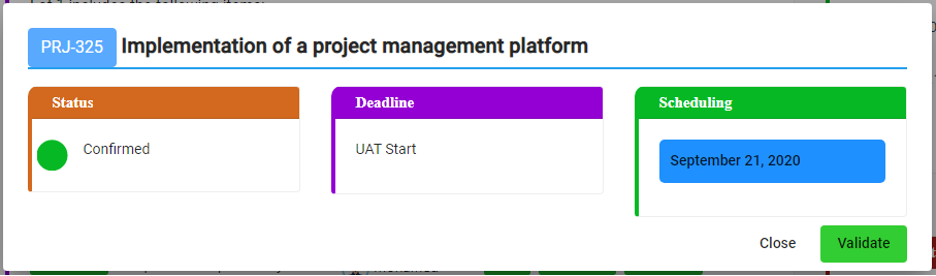
\includegraphics{figures/33anis24.png}
    \caption{Interface de planification de projet}
    \label{fig:interface_planification}
\end{figure}\newpage
\subsubsection{Interface d’un risque }
\hspace{4mm}La figure suivante présente les détails d’un risque.
\begin{figure}[h]
    \centering
    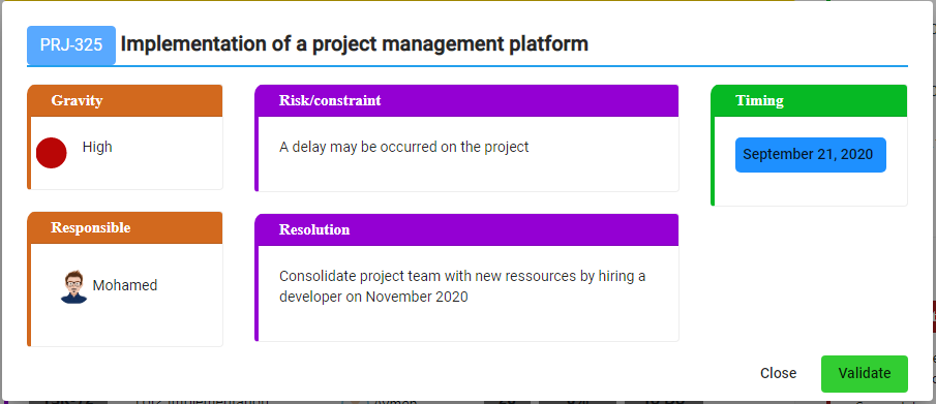
\includegraphics{figures/33anis25.png}
    \caption{Interface d’un risque}
    \label{fig:interface_risque}
\end{figure}\newpage
\subsection{Interface d’une tâche }
\hspace{4mm}La figure suivante présente les détails d’une tâche. Cette interface offre aussi la possibilité de consulter les détails d’une planification et les détails d’un risque.
\begin{figure}[h]
    \centering
    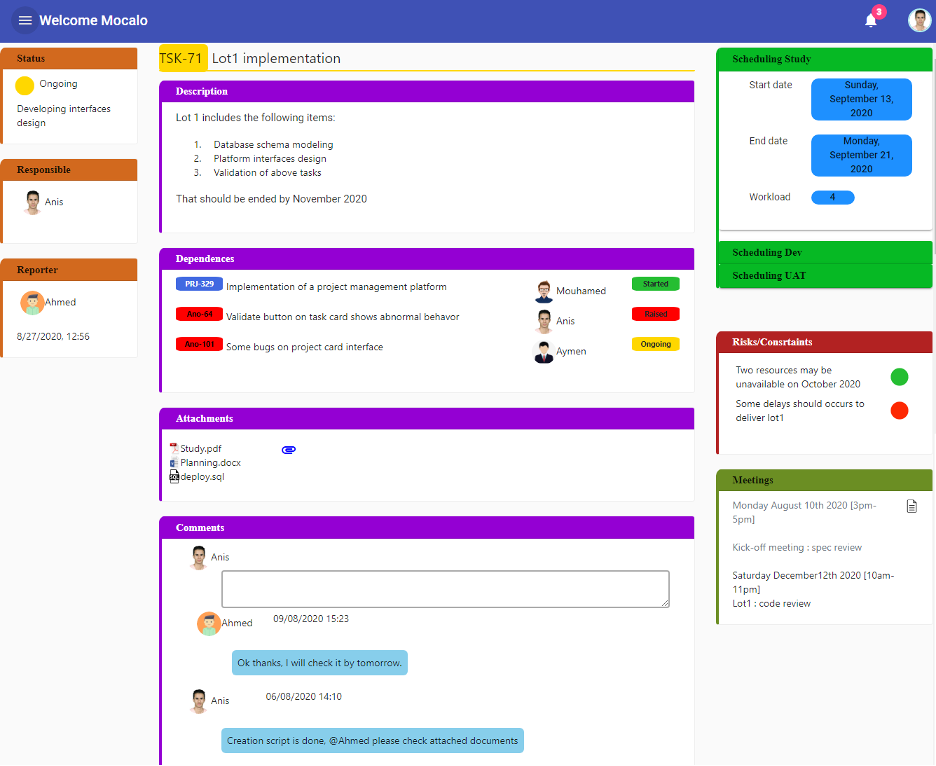
\includegraphics{figures/33anis26.png}
    \caption{Interface d’une tâche}
    \label{fig:interface_tache}
\end{figure}\newpage
\subsection{	Interface d'une anomalie }
\hspace{4mm}La figure suivante présente les détails d’une anomalie. Cette interface offre aussi la possibilité de consulter les détails d’une planification.
\begin{figure}[h]
    \centering
    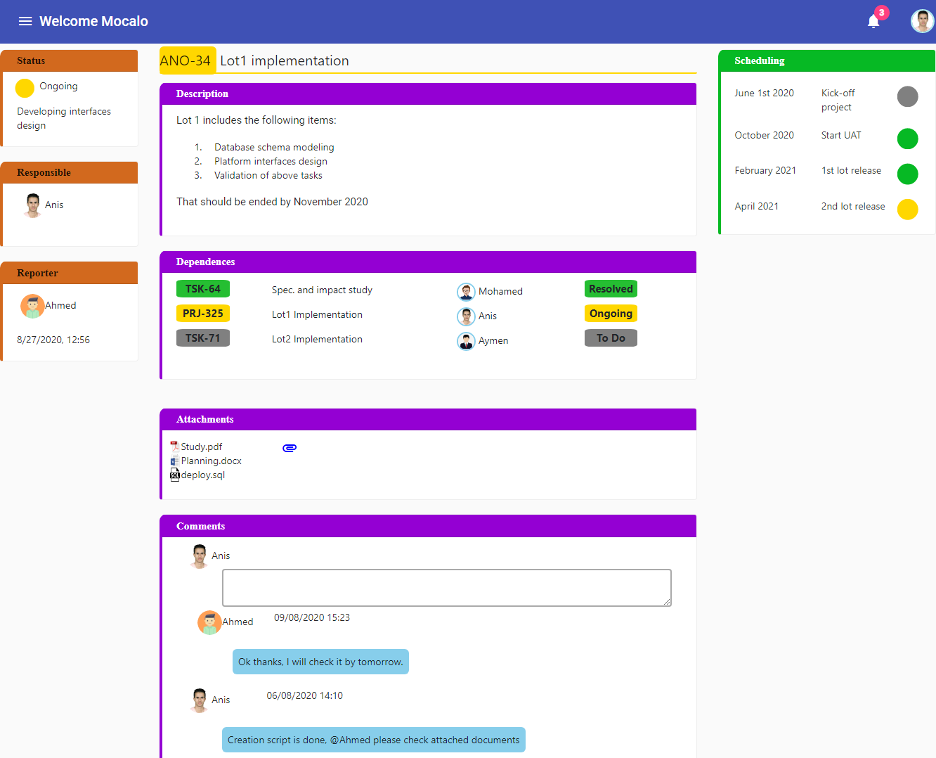
\includegraphics{figures/33anis27.png}
    \caption{Interface de l’anomalie}
    \label{fig:interface_anomalie}
\end{figure}\newpage
\subsection{	Interface d’une libération de tâche}
\hspace{4mm}La figure suivante présente les détails d’une libération de tâche. Cette interface offre aussi la possibilité de consulter les détails d’une planification.
\begin{figure}[h]
    \centering
    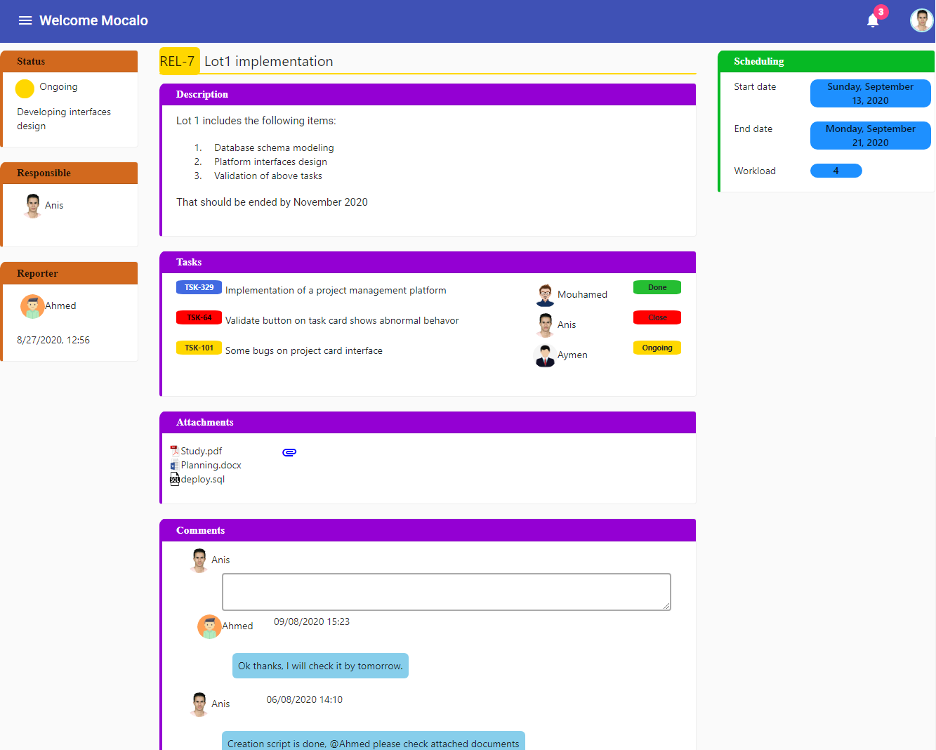
\includegraphics{figures/33anis28.png}
    \caption{Interface d’une libération}
    \label{fig:interface_liberation}
\end{figure}\newpage
\subsection{	Interface d'un emploi du temps  }
\hspace{4mm}La figure suivante présente l’interface d'un emploi du temps.
\begin{figure}[h]
    \centering
    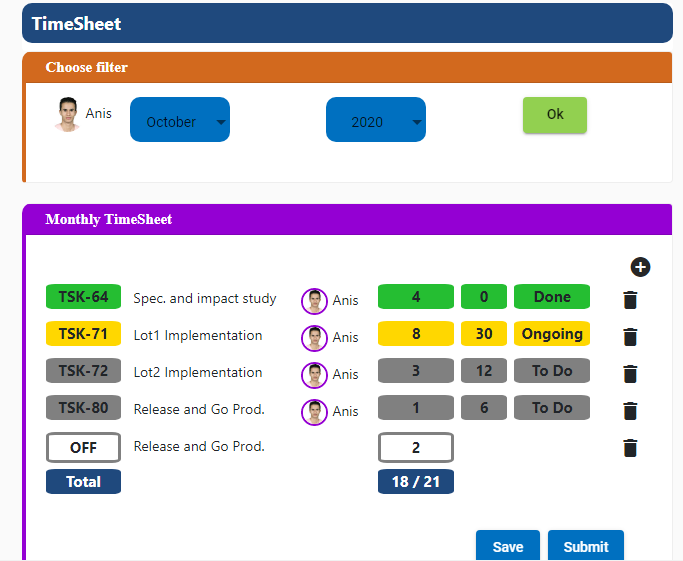
\includegraphics[scale=0.5]{figures/3333anis7.png}
    \caption{Interface d'un emploi du temps}
    \label{fig:interface_timesheet}
\end{figure}
\subsection{Interface de prévision de congé}
\hspace{4mm}La figure suivante présente l’interface de la liste de prévision de congé.
\begin{figure}[h]
    \centering
    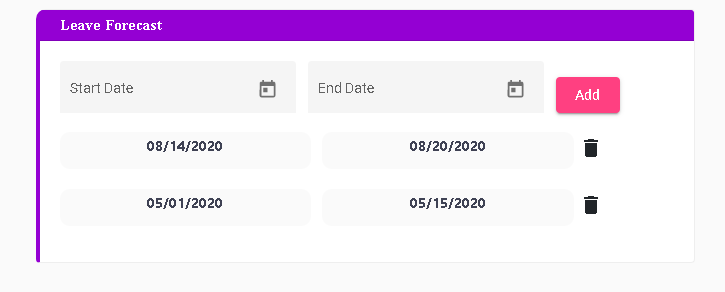
\includegraphics[scale=0.65]{figures/a5.png}
    \caption{Interface de prévision de congé}
    \label{fig:interface_congé}
\end{figure}\newpage
\subsection{	Interfaces de réunion}
\hspace{4mm}Cette interface permet à l’utilisateur de fixer une date de réunion. \newline
\begin{figure}[h]
    \centering
    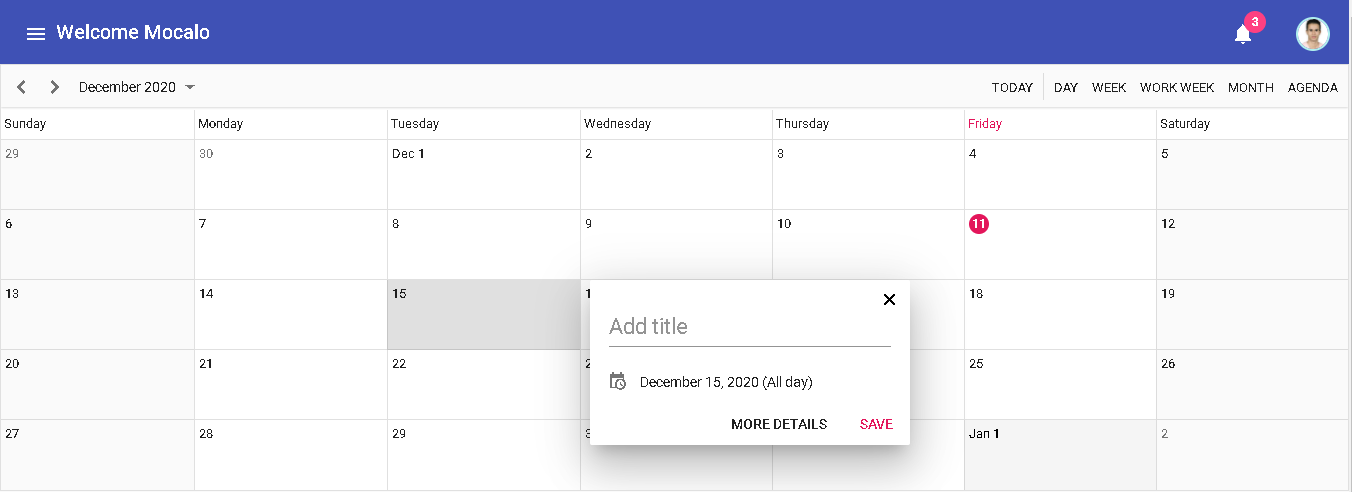
\includegraphics[scale=0.35]{figures/a6.png}
    \caption{Interface de sélection d'une date de  réunion}
    \label{fig:interface_reunion}
\end{figure}\newline
\hspace{4mm}La figure suivante présente l’interface de création d'une réunion.  \newline
\begin{figure}[h]
    \centering
    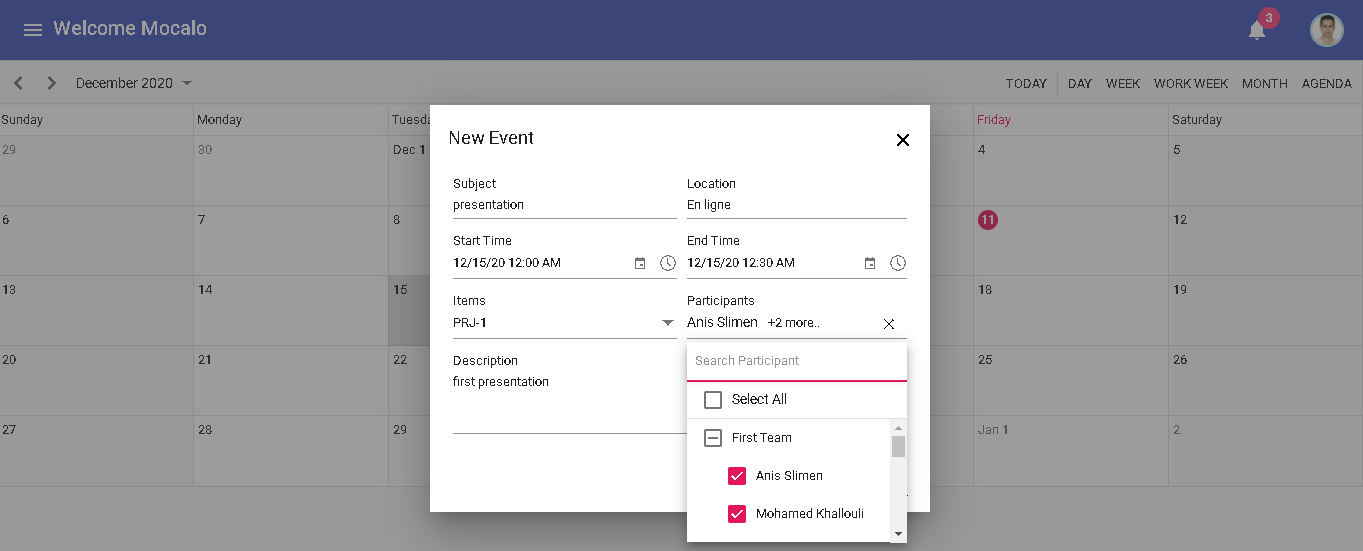
\includegraphics[scale=0.35]{figures/a7.png}
    \caption{Interface de création d'une réunion}
    \label{fig:interface_creation_reunion}
\end{figure}\newpage
\par La figure suivante présente l’interface résultat de la création d'une réunion.
\begin{figure}[h]
    \centering
    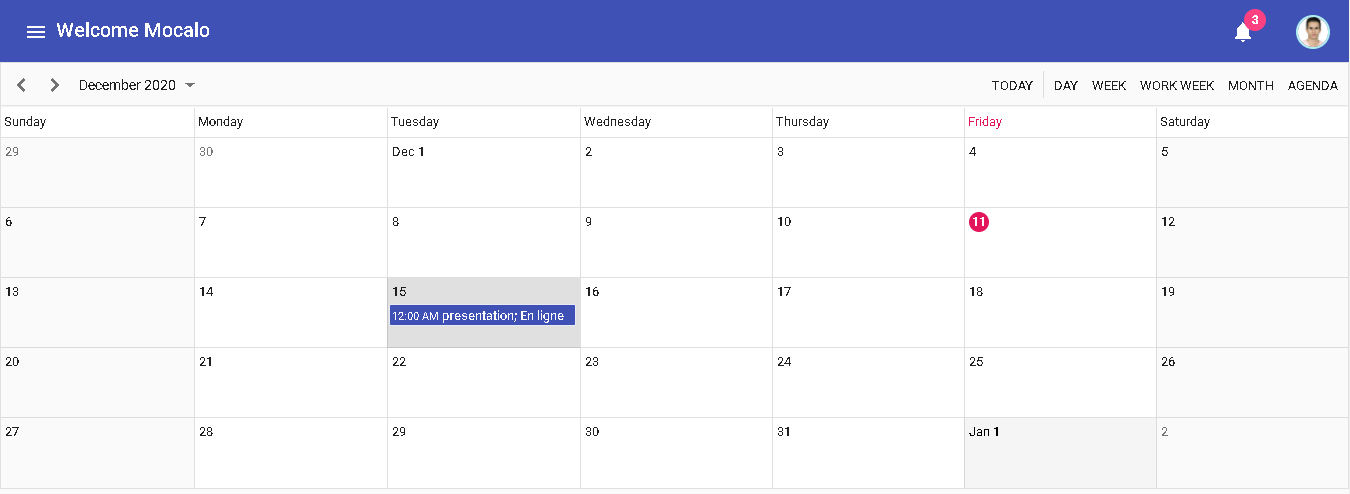
\includegraphics[scale=0.35]{figures/a8.png}
    \caption{Interface résultat de la création d'une réunion}
    \label{fig:interface_resultcreation_reunion}
\end{figure}
\subsection{	Interface de Notification }
\hspace{4mm}La figure suivante présente l’interface de Notification.
\begin{figure}[h]
    \centering
    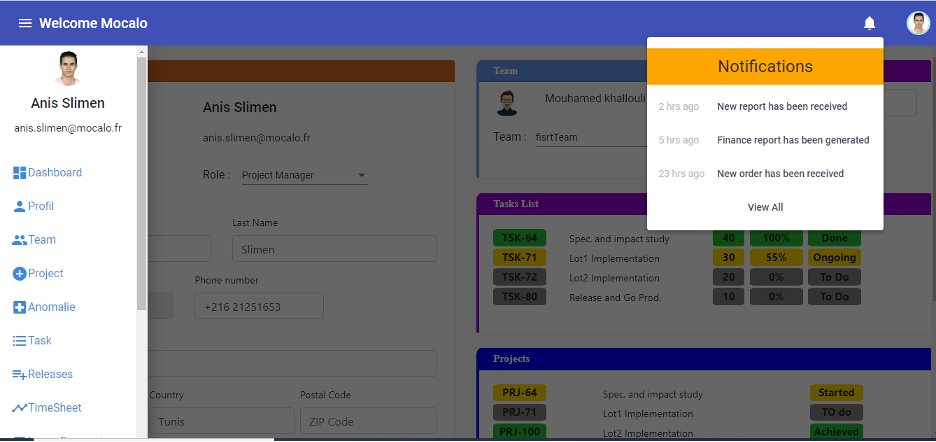
\includegraphics{figures/33anis3'.png}
    \caption{Interface de Notification}
    \label{fig:interface_notification}
\end{figure}
\section*{	Conclusion}
\hspace{4mm} 
Dans ce dernier chapitre, nous avons décrit l'environnement du travail et présenté les principales interfaces de l'application réalisée.
